
\documentclass[a4paper]{article}
\usepackage[utf8]{inputenc}

\usepackage[english,german]{babel} 
\usepackage[utf8]{inputenc}

\usepackage{alltt}
\usepackage{amsmath}
\usepackage{amssymb}
\usepackage{amsthm}
\usepackage{color}
\usepackage{enumitem}
\usepackage{epsfig}
\usepackage{fancyhdr}
\usepackage{float}
\usepackage{framed}
\usepackage{graphicx} 
\usepackage{graphics}
\usepackage{hyperref}
\usepackage{listings}
\usepackage{multirow}
\usepackage{tabularx}
\usepackage{textcomp}
\usepackage{tikz}
\usepackage{url}
\usepackage{vmargin}
\usepackage{xspace}
\usepackage{comment}
\usetikzlibrary{calc,trees,positioning,arrows,chains,shapes.geometric,%
    decorations.pathreplacing,decorations.pathmorphing,shapes,%
    matrix,shapes.symbols,topaths,matrix}
\newcommand{\question}[2][0]{\section{{#2} \hfill ({#1} P.)}}
\setpapersize{A4}
\setmargins{2.5cm}{2.0cm}% % linker & oberer Rand
         {16cm}{22cm}%   % Textbreite und -hoehe
           {48pt}{36pt}%   % Kopfzeilenhoehe und -abstand
           {0pt}{30pt}%    % \footheight (egal) und Fusszeilenabstand

\frenchspacing
\pagestyle{fancy}
\sloppy

\newcommand{\hide}[1]{}

\markright{Kopfzeile}


\tikzset{
>=stealth',
  punktchain/.style={
    rectangle,
    rounded corners,
    % fill=black!10,
    draw=black, very thick,
    text width=10em,
    minimum height=3em,
    text centered,
    on chain},
  line/.style={draw, thick, <-},
  element/.style={
    tape,
    top color=white,
    bottom color=blue!50!black!60!,
    minimum width=8em,
    draw=blue!40!black!90, very thick,
    text width=10em,
    minimum height=3.5em,
    text centered,
    on chain},
  every join/.style={->, thick,shorten >=1pt},
  decoration={brace},
  tuborg/.style={decorate},
  tubnode/.style={midway, right=2pt},
}


\setlength{\parindent}{0pt}
\setlength{\parskip}{5pt}
\fboxsep1.5mm


\lstdefinestyle{mystyle}{
    backgroundcolor=\color{white},   
    commentstyle=\color{codegray},
    keywordstyle=\bf \ttfamily \color{codepurple},
    numberstyle=\tiny\color{codegray},
    stringstyle=\color{codegreen},
    basicstyle=\footnotesize,
    breakatwhitespace=false,         
    breaklines=true,                 
    captionpos=b,                    
    keepspaces=true,                 
    numbers=left,                    
    numbersep=5pt,                  
    showspaces=false,                
    showstringspaces=false,
    showtabs=false,                  
    tabsize=8,
    keepspaces,
    extendedchars=true, 
      upquote=true,
    columns=fixed,
    showstringspaces=false,
    extendedchars=true,
    breaklines=true,
    frame=single,
    showspaces=false,
    showstringspaces=false,
    rulecolor=\color{white},
}

\lstdefinelanguage{sql}[]{}{
        %tag=[s]<>,      % =*: also apply styles within tag, =**: cumulate styles
        morekeywords={sql, VIEW, AS, FROM, SELECT, WHERE, FUNCTION, BOOLEAN, RETURNS, DETERMINISTIC, RETURN, REFERENCES, WITH, SEQUENCE, TRUNCATE, START, CREATE, AS, LANGUAGE, FUNCTION, CURSOR, PREPARE, OPEN, USING, CLOSE, DECLARE, END, BEGIN, EXEC, SQL, CONNECT TO, DISCONNECT, COMMIT, LOOP, IF, THEN, ELSE, WHILE, BREAK, EXIT, INSERT, INTO, VALUES, UPDATE, SET, TABLE, PRIMARY, KEY, AND, UNION, ALL, JOIN, ON, GROUP, BY, MATERIALIZED, INT, DATE, COUNT, ORDER, OVER, PARTITION, ASC, DESC, VARCHAR, NOT, NULL, PRIMARY, KEY, DECIMAL, SUM, AVG, ROWS, BETWEEN, PRECEDING, CURRENT, ROW, INSTEAD, TRIGGER, OF, FOR, EACH, EXECUTE, PROCEDURE, DISTINCT, HAVING, LIMIT},
morestring=[s]{'}{'},
morecomment=[l]{--}
        %sensitive=false
}

\lstset{style=mystyle,numbers=none,basicstyle=\ttfamily,upquote=true}

 
\definecolor{codegreen}{rgb}{0,0.6,0}
\definecolor{codegray}{rgb}{0.5,0.5,0.5}
\definecolor{codepurple}{rgb}{0.38,0,0.72}
\definecolor{backcolour}{rgb}{0.95,0.95,0.92}
\definecolor{backcolourSingleCode}{rgb}{0.95,0.95,0.92}

\newcommand{\subtitle}{\textbf{Exercise 7}}
\newcommand{\outdate}{04.12.2023}
\newcommand{\duedate}{11.12.2023 12:00 MEZ}
\newcommand{\video}{036}

\usepackage{tkz-euclide}
\begin{document}

\lhead{\begin{tabular}{l}
{\bf Database Systems WS 2023/24}\\
{\bf \subtitle: Distributed \outdate, Due \duedate}\\
{Submitted by }
\end{tabular}
}
\rhead{}

\question[1]{Space filling curves for NN-queries}
\begin{enumerate}
  \item 
  Implement space-filling z-curves in a language of your choice.
Your program has to take two files which contain points as input.
The first file contains all the points of the base data set, while the second file contains query points.
The program has to calculate and display:
\begin{itemize}
\item The k-NN, of each query point, in the base data set, based on the actual distance.
\item The k-NN, of each query point, in the base data set, based on the z-curve distance.
\end{itemize}

You can use the template in OLAT, which already parses the files and provides utility classes.
Submit the code and the output of your program when executed with $k = 3$ and the two data files provided in OLAT.
If you do not use the template, also submit instructions on how to compile and execute your program.

\textit{Note: } If you use code from external sources, provide the source as a comment.\\

{\bf Solution:}\\
\begin{figure}[H]
  \centering
  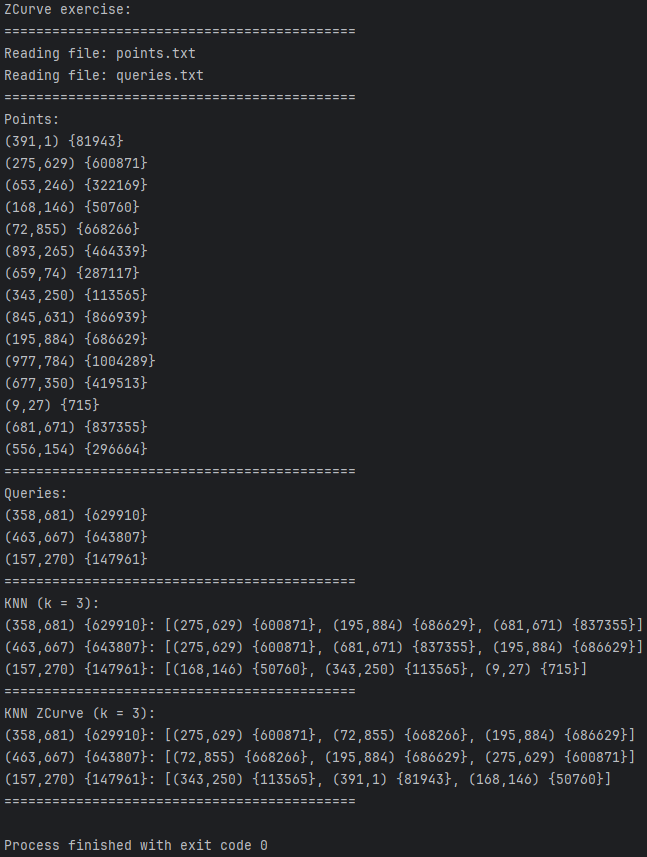
\includegraphics[scale = 0.6]{ZCurveOutput.PNG}
\end{figure}

\item
Which differences can you see between the two results of your implementation?
Explain why are or why are not the results the same.\\\\
{\bf Solution:}\\
Some of the actual k-NN are matching the k-NN according to the z-curve value, but not all of them.
The z-curve mapping is only an approximation of the actual k-NN.\\

Let's have a look at the points $A(0,0)$, $B(1,0)$, and $C(0,1)$. The real distance between $A$ and $B$ is $1$.
Also, the z-value is $1$ in this case. The real distance between $A$ and $C$ is also $1$, but in this case, 
the z-value is $2$. Because of the shape of the z-curve, the z-value is only an estimation of the real distance.

\end{enumerate}

\newpage

\question[1]{R Tree}

Given the following two-dimensional objects:

\begin{center}
  \begin{tikzpicture}

    \draw[help lines, color=gray!30, dashed] (0,0) grid (10,6);

    \draw (0,0) -- coordinate (x axis mid) (10,0);
    \draw (0,0) -- coordinate (y axis mid) (0,6);

    \foreach \x in {0,...,10} \draw (\x,1pt) -- (\x,-3pt) node[anchor=north] {\x};
    \foreach \y in {0,...,6}  \draw (1pt,\y) -- (-3pt,\y) node[anchor=east] {\y};

    \tkzDefPoint(1,1){f1a};
    \tkzDefPoint(1,5){f1b};
    \tkzDefPoint(2,5){f1c};
    \tkzDefPoint(3,3){f1d};
    \tkzDefPoint(2,1){f1e};

    \tkzDrawPolygon[fill=purple!30](f1a,f1b,f1c,f1d,f1e);
    \node at (barycentric cs:f1a=1,f1b=1,f1c=1,f1d=1,f1e=1) {F1};

    \draw[fill=yellow!30] (4,5) circle (1);
    \node at (4,5) {F2};

    \tkzDefPoint(4,2){f3a};
    \tkzDefPoint(5,3){f3b};
    \tkzDefPoint(6,3){f3c};
    \tkzDefPoint(6,2){f3d};
    \tkzDefPoint(5,1){f3e};

    \tkzDrawPolygon[fill=green!30](f3a,f3b,f3c,f3d,f3e);
    \node at (barycentric cs:f3a=1,f3b=1,f3c=1,f3d=1,f3e=1) {F3};

    \draw[fill=blue!30] (8,2) circle (1);
    \node at (8,2) {F4};

    \tkzDefPoint(6,4){f5a};
    \tkzDefPoint(9,4){f5b};
    \tkzDefPoint(9,6){f5c};
    \tkzDefPoint(8,6){f5d};
    \tkzDefPoint(8,5){f5e};
    \tkzDefPoint(6,5){f5f};

    \tkzDrawPolygon[fill=red!30](f5a,f5b,f5c,f5d,f5e,f5f);
    \node at (barycentric cs:f5a=3,f5b=3,f5c=1,f5d=1,f5e=1,f5f=1) {F5};
  \end{tikzpicture}
\end{center}

For the following R tree operations, explain exactly which steps are performed:

\begin{enumerate}
\item
  {\em Store the objects F1, F2, F3, F4, F5 in an initially empty R tree}.
  One node fits 1--2 entries.\\\\
  {\bf Solution:}\\
  The objects get inserted one after the other in theory they can be inserted in any node.
  I decided for the following insertion order: F1, F5, F4, F2, F3.
  F1 and F5 get inserted into the tree.\\
\begin{center}
  \begin{tikzpicture}[level distance=1.5cm,
    level 1/.style={sibling distance=3cm}]
    \node[draw]{$R1|R2$}
      child{node[draw]{$F1|null$}}
      child{node[draw]{$F5|null$}};
  \end{tikzpicture}
\end{center}
  

  R1 is the smalest rectangle that fits around F1 and R2 is the smalest rectangle that fits arround F5
  Insertion of F4:\\
  Calculate the arrea differences of R1 if F4 gets inserted into R1 and calculate the area difference of R2 if F4 gets inserted.\\\\
  \begin{center}
    $A_{R1} = 8 \cdot 4 - 2 \cdot 4 = 24$\\
    $A_{R2} = 5 \cdot 3 - 6 \cdot 4 = 9$
  \end{center}
    
  Insert F4 int R2 because the area increase is smaler then when inserted into R2\\\\
  \begin{center}
    \begin{tikzpicture}[level distance=1.5cm,
      level 1/.style={sibling distance=3cm}]
      \node[draw]{$R1|R2$}
        child{node[draw]{$F1|null$}}
        child{node[draw]{$F5|F4$}};
    \end{tikzpicture}
  \end{center}
  Insertion of F2:\\
  Calculate the arrea differences of R1 if F2 gets inserted into R1 and calculate the area difference of R2 if F2 gets inserted.\\\\
  \begin{center}
    $A_{R1} = 4 \cdot 5 - 2 \cdot 4 = 12$\\
    $A_{R2} = 5 \cdot 3 - 3 \cdot 5 = 15$
  \end{center}
    
  Insert F2 int R1 because the area increase is smaler then when inserted into R1\\\\
  \begin{center}
    \begin{tikzpicture}[level distance=1.5cm,
      level 1/.style={sibling distance=3cm}]
      \node[draw]{$R1|R2$}
        child{node[draw]{$F1|F2$}}
        child{node[draw]{$F5|F4$}};
    \end{tikzpicture}
  \end{center}
  Insertion of F3:\\
  Calculate the area differences of R1 if F2 gets inserted into R1 and calculate the area difference of R2 if F2 gets inserted.\\\\
  \begin{center}
    $A_{R1} = 5 \cdot 5 - 4 \cdot 5 = 5$\\
    $A_{R2} = 5 \cdot 5 - 3 \cdot 5 = 10$
  \end{center}
  Insert F2 int R1 because the area increase is smaler then when inserted into R1. The maximum of objects in R1 is already reached. 
  In order to insert F2 R1 needs to be split into two rectangles. The size of the two newly created rectangels R3 and R4 should be minimal in the optimal case.\\
  Calculation of the area of all posible split combinations:\\\\
  \begin{center}
    $R3[F1, F2], R4[F3]$ $A = 4 \cdot 5 + 2 \cdot 2 = 24$\\
    $R3[F1, F3], R4[F2]$ $A = 5 \cdot 4 + 2 \cdot 2 = 24$\\
    $R3[F3, F2], R4[F1]$ $A = 3 \cdot 5 + 2 \cdot 4 = 23$
  \end{center}
    
    According to the Calculation the last option is to optimal one because the area of R3 and R4 will be minimal. The R-Tree looks now like:\\\\
    \begin{center}
      \begin{tikzpicture}[level distance=1.5cm,
        level 1/.style={sibling distance=3cm},
        level 2/.style={sibling distance=3cm}]
        \node[draw]{$R1|R2$}
          child
          { node[draw]{$R3|R4$}
            child{node[draw]{$F3|F2$}}
            child{node[draw]{$F1|null$}}
          }
          child{node[draw]{$F5|F4$}};
      \end{tikzpicture}
    \end{center}
    
    In the two dimensional plane the R-Tree looks like the following:
    \begin{center}
      \begin{tikzpicture}
    
        \draw[help lines, color=gray!30, dashed] (0,0) grid (10,6);
    
        \draw (0,0) -- coordinate (x axis mid) (10,0);
        \draw (0,0) -- coordinate (y axis mid) (0,6);
    
        \foreach \x in {0,...,10} \draw (\x,1pt) -- (\x,-3pt) node[anchor=north] {\x};
        \foreach \y in {0,...,6}  \draw (1pt,\y) -- (-3pt,\y) node[anchor=east] {\y};
    
        \tkzDefPoint(1,1){f1a};
        \tkzDefPoint(1,5){f1b};
        \tkzDefPoint(2,5){f1c};
        \tkzDefPoint(3,3){f1d};
        \tkzDefPoint(2,1){f1e};
    
        
        \tkzDrawPolygon[fill=purple!30](f1a,f1b,f1c,f1d,f1e);
        \node at (barycentric cs:f1a=1,f1b=1,f1c=1,f1d=1,f1e=1) {F1};
    
        \draw[fill=yellow!30] (4,5) circle (1);
        \node at (4,5) {F2};
    
        \tkzDefPoint(4,2){f3a};
        \tkzDefPoint(5,3){f3b};
        \tkzDefPoint(6,3){f3c};
        \tkzDefPoint(6,2){f3d};
        \tkzDefPoint(5,1){f3e};
    
        \tkzDrawPolygon[fill=green!30](f3a,f3b,f3c,f3d,f3e);
        \node at (barycentric cs:f3a=1,f3b=1,f3c=1,f3d=1,f3e=1) {F3};
    
        \draw[fill=blue!30] (8,2) circle (1);
        \node at (8,2) {F4};
    
        \tkzDefPoint(6,4){f5a};
        \tkzDefPoint(9,4){f5b};
        \tkzDefPoint(9,6){f5c};
        \tkzDefPoint(8,6){f5d};
        \tkzDefPoint(8,5){f5e};
        \tkzDefPoint(6,5){f5f};
    
        \tkzDrawPolygon[fill=red!30](f5a,f5b,f5c,f5d,f5e,f5f);
        \node at (barycentric cs:f5a=3,f5b=3,f5c=1,f5d=1,f5e=1,f5f=1) {F5};

        \tkzDefPoint(1,1){R1a};
        \tkzDefPoint(6,1){R1b};
        \tkzDefPoint(6,6){R1c};
        \tkzDefPoint(1,6){R1d};
    
        \tkzDrawPolygon[line width=0.6mm, red](R1a, R1b, R1c, R1d);
        \node at (2,5.5) {\textcolor{red}{R1}};

        \tkzDefPoint(6,1){R2a};
        \tkzDefPoint(9,1){R2b};
        \tkzDefPoint(9,6){R2c};
        \tkzDefPoint(6,6){R2d};
    
        \tkzDrawPolygon[line width=0.6mm, red](R2a, R2b, R2c, R2d);
        \node at (7,5.5) {\textcolor{red}{R2}};

        \tkzDefPoint(3,1){R3a};
        \tkzDefPoint(6,1){R3b};
        \tkzDefPoint(6,6){R3c};
        \tkzDefPoint(3,6){R3d};
    
        \tkzDrawPolygon[line width=0.2mm, green](R3a, R3b, R3c, R3d);
        \node at (5.5,5.5) {\textcolor{green}{R3}};

        \tkzDefPoint(1,1){R4a};
        \tkzDefPoint(3,1){R4b};
        \tkzDefPoint(3,5){R4c};
        \tkzDefPoint(1,5){R4d}; 
    
        \tkzDrawPolygon[line width=0.2mm, green](R4a, R4b, R4c, R4d);
        \node at (2.6,4.5) {\textcolor{green}{R4}};
      \end{tikzpicture}
    \end{center}
\item
  {\em Find all objects, containing the point (6,2).}\\\\
  {\bf Solution:}\\\\
  Step by step execution:\\
  \subitem
  Scan the root of the tree (R1,R2)
  \subitem
  Check if (6,2) is in R1 $\Rightarrow$ true $\Rightarrow$ put R3 and R4 in the que
  \subitem
  Check if (6,2) is in R2 $\Rightarrow$ true $\Rightarrow$ put F5 and F4 in the que
  \subitem
  Check if (6,2) is in R3 $\Rightarrow$ true $\Rightarrow$ put F2 and F3 in the que
  \subitem
  Check if (6,2) is in R4 $\Rightarrow$ false
  \subitem
  Check if (6,2) is in F5 $\Rightarrow$ false
  \subitem
  Check if (6,2) is in F4 $\Rightarrow$ false
  \subitem
  Check if (6,2) is in F2 $\Rightarrow$ false
  \subitem
  Check if (6,2) is in F3 $\Rightarrow$ true $\Rightarrow$ leafnode $\Rightarrow$ add F3 to the query result
  \subitem
  (6,2) is only in object F3

\item
{\em Find all objects that are positioned completely in the rectangle $Q$, which is defied by the points $(2, 1) (9, 3)$.}

\item
  {\em Find all objects, intersecting with $Q'$: $(2,2) (4,4)$.}

  We assume that sharing exactly one point, also counts as intersecting.

\end{enumerate}

\question[1]{Index Structures in Metric Space}

Show, for each of the following distance functions, that the properties for being a metric are fulfilled, or provide a counterexample.

    \begin{enumerate}

   \item\label{l1} 
   For two vectors (or points) $a=(x_a, y_a)$ and $b=(x_b, y_b)$:

 $d(a, b) \mapsto | x_a - x_b | + | y_a - y_b |$.  

  \item\label{l2} 
For two vectors (or points) $a=(x_a, y_a)$ and $b=(x_b, y_b)$:
 $d(a, b) \mapsto ( x_a - x_b )^2 + ( y_a - y_b )^2$.

      \item\label{l3} 
      For two strings $s_1$ and $s_2$, where $S$ is the set of characters of the string (e.g.: $S(\text{``Codd''}) = \{\text{`C', `o', `d'}\}$):
      $d(s_1, s_2) \mapsto 2* |S(s_1) \cap S(s_2)| \, / \, (|S(s_1)| + |S(s_2)|)$.\\

    \end{enumerate}

\newpage
\question[1]{Misc Metric Indexing}

  Below are the points used for the following questions:
\[
1: (17, 29) \hspace{5mm}
2: (4, 21) \hspace{5mm}
3: (20, 29) \hspace{5mm}
4: (4, 36) \hspace{5mm}
5: (35, 28)
\]
\[
6: (39, 22) \hspace{5mm}
7: (30, 5) \hspace{5mm}
8: (8, 36) \hspace{5mm}
9: (6, 2) \hspace{5mm}
10: (20, 4)
\]
\[
11: (4, 6) \hspace{5mm}
12: (29, 32) \hspace{5mm}
13: (22, 33) \hspace{5mm}
14: (38, 18) \hspace{5mm}
15: (16, 25)
\]

\begin{enumerate}
  \item \textbf{GH Tree partitioning:} 
    Create a GH partitioning, such that the leaf nodes of the tree have at most $2$ elements.
    Draw the tree and draw the partitioning into the plot below.

\begin{center}
\begin{tikzpicture}
\begin{axis}[ymin = 0, xmin = 0]
  \addplot+[nodes near coords,only marks,
    point meta=explicit symbolic] 
  coordinates {
(17, 29) [1] 
(4, 21) [2] 
(20, 29) [3] 
(4, 36) [4] 
(35, 28) [5] 
(39, 22) [6] 
(30, 5) [7] 
(8, 36) [8] 
(6, 2) [9] 
(20, 4) [10]
(4, 6) [11]
(29, 32) [12]
(22, 33) [13]
(38, 18) [14]
(16, 25) [15]
  };
\end{axis}
\end{tikzpicture}
\end{center}

\item \textbf{VP Tree:}
Given the following VP tree, search for query point (25,4) with $\varepsilon = 11$.
Describe which parts of the tree you pruned and why.

\begin{center}
  \begin{tikzpicture}[every text node part/.style={align=center},level 1/.style={sibling distance=60mm},level 2/.style={sibling distance=30mm},level 3/.style={sibling distance=15mm}]
\node { 7\\(30, 5)\\$r=26.01$ } child {node { 14\\(38, 18)\\$r=21.95$ } child {node { 6\\(39, 22)\\$r=13.73$ } child {node { 5\\(35, 28) }} child {node { 3\\(20, 29) }}} child {node { 15\\(16, 25)\\$r=23.23$ } child {node { 10\\(20, 4) }} child {node { 9\\(6, 2) }}}} child {node { 1\\(17, 29)\\$r=13.57$ } child {node { 8\\(8, 36)\\$r=17.85$ } child {node { 13\\(22, 33) }} child {node { 12\\(29, 32) }}} child {node { 4\\(4, 36)\\$r=22.5$ } child {node { 2\\(4, 21) }} child {node { 11\\(4, 6) }}}};
  \end{tikzpicture}
  \end{center}

\end{enumerate}

\end{document}
